\documentclass{beamer}
\usepackage[unilu,en]{collegeBeamer}
\usepackage[usenames,dvipsnames]{xcolor}
\setbeamertemplate{footline}[frame number]
\usepackage{graphicx}
\usepackage{tikz}
\usetikzlibrary{calc, arrows.meta, positioning, shapes.geometric, fit, backgrounds, decorations.pathreplacing}
\usepackage{listings}
\usepackage{fontawesome5}
\usepackage{hyperref}

% Code listing style
\lstset{
    basicstyle=\ttfamily\scriptsize,
    breaklines=true,
    frame=single,
    backgroundcolor=\color{gray!10}
}

% meta-data
\title{Pulse of Engagement}
\subtitle{Visual Analytics for Economic Health in Engagement, OH\\VAST Challenge 2022 -- Challenge 3}
\author{Thomas Gantz \and Michal Sterzel \and Jan Marxen}
\date{December 2025}
\themecolor{50,50,50}

% document body
\begin{document}

% Custom title page with Ohio map
\begin{frame}[plain]
    \centering
    \vspace{0.3cm}
    {\Huge\bfseries Pulse of Engagement}\\[0.25cm]
    {\large Visual Analytics for Economic Health in Engagement, OH}\\[0.1cm]
    {\small VAST Challenge 2022 -- Challenge 3}\\[0.4cm]
    {\normalsize Thomas Gantz \quad Michal Sterzel \quad Jan Marxen}\\[0.2cm]
    {\small December 2025}\\[0.3cm]
    \includegraphics[width=0.35\textwidth]{img/ohio-map-on-white-background-free-vector.jpg}
\end{frame}

% ==============================================================================
\section{Introduction}
% ==============================================================================

\begin{frame}{VAST Challenge 2022 -- Challenge 3}
    \begin{columns}
        \begin{column}{0.55\textwidth}
            \textbf{The Challenge}
            \begin{itemize}
                \item Analyze economic health of a fictional city
                \item Dataset: $\sim$120 million data points
                \item 15 months of 5-minute granularity data
            \end{itemize}
            
            \vspace{10pt}
            \textbf{Three Questions}
            \begin{enumerate}
                \item Business Prosperity
                \item Resident Financial Health
                \item Employer Health \& Turnover
            \end{enumerate}
        \end{column}
        \begin{column}{0.42\textwidth}
            \centering
            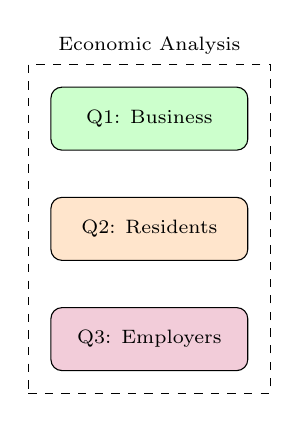
\begin{tikzpicture}[
                scale=0.7,
                box/.style={rectangle, draw, rounded corners, fill=blue!20, minimum width=2.5cm, minimum height=0.8cm, font=\scriptsize, align=center}
            ]
                \node[box, fill=green!20] (q1) at (0,2) {Q1: Business};
                \node[box, fill=orange!20] (q2) at (0,0) {Q2: Residents};
                \node[box, fill=purple!20] (q3) at (0,-2) {Q3: Employers};
                
                \node[rectangle, draw, dashed, fit=(q1)(q2)(q3), inner sep=8pt, label=above:{\scriptsize Economic Analysis}] {};
            \end{tikzpicture}
        \end{column}
    \end{columns}
\end{frame}

\begin{frame}{Our Solution: Pulse of Engagement}
    \centering
    \vspace{5pt}
    
    % TODO: Replace with actual screenshot of the main dashboard
    \fbox{\parbox{0.85\textwidth}{\centering\vspace{2cm}\textbf{[SCREENSHOT: Main Dashboard Overview]}\\\small Show the tabbed interface with all three question areas\vspace{2cm}}}
    
    \vspace{10pt}
    \small
    Interactive web application built with \textbf{React + D3.js} frontend and \textbf{Python Flask} backend
\end{frame}

% ==============================================================================
\section{Question 1: Business Prosperity}
% ==============================================================================

\begin{frame}{Q1: Business Prosperity}
    \centering
    \vspace{1cm}
    
    {\Large \textbf{[PLACEHOLDER FOR THOMAS]}}
    
    \vspace{1cm}
    
    \begin{itemize}
        \item Which businesses are thriving vs. struggling?
        \item Revenue trends over time
        \item Market share evolution
    \end{itemize}
    
    \vspace{1cm}
    
    % TODO: Add screenshots of business visualizations
    \fbox{\parbox{0.7\textwidth}{\centering\vspace{1.5cm}\textbf{[SCREENSHOT: Business Visualizations]}\vspace{1.5cm}}}
\end{frame}

\begin{frame}{Q1: Key Findings}
    \centering
    \vspace{1cm}
    
    {\Large \textbf{[PLACEHOLDER FOR THOMAS]}}
    
    \vspace{1cm}
    
    \begin{columns}
        \begin{column}{0.48\textwidth}
            \textbf{Prosperous Businesses}
            \begin{itemize}
                \item [To be filled by teammate]
            \end{itemize}
        \end{column}
        \begin{column}{0.48\textwidth}
            \textbf{Struggling Businesses}
            \begin{itemize}
                \item [To be filled by teammate]
            \end{itemize}
        \end{column}
    \end{columns}
\end{frame}

% ==============================================================================
\section{Question 2: Resident Financial Health}
% ==============================================================================

\begin{frame}{Q2: Analysis Approach}
    \vspace{-5pt}
    \textbf{Three Complementary Lenses}
    \vspace{5pt}
    \begin{columns}[T]
        \begin{column}{0.32\textwidth}
            \centering
            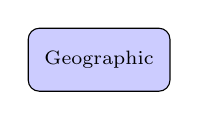
\begin{tikzpicture}
                \node[rectangle, draw, rounded corners, fill=blue!20, minimum width=1.8cm, minimum height=0.8cm, font=\scriptsize, align=center] {Geographic};
            \end{tikzpicture}
            \footnotesize
            \begin{itemize}\setlength{\itemsep}{1pt}
                \item Building heatmap
                \item Savings by location
                \item Identify red zones
            \end{itemize}
        \end{column}
        \begin{column}{0.32\textwidth}
            \centering
            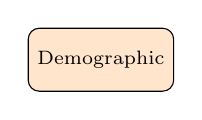
\begin{tikzpicture}
                \node[rectangle, draw, rounded corners, fill=orange!20, minimum width=1.8cm, minimum height=0.8cm, font=\scriptsize, align=center] {Demographic};
            \end{tikzpicture}
            \footnotesize
            \begin{itemize}\setlength{\itemsep}{1pt}
                \item Wage vs. cost
                \item K-Means clustering
                \item Education link
            \end{itemize}
        \end{column}
        \begin{column}{0.32\textwidth}
            \centering
            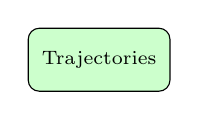
\begin{tikzpicture}
                \node[rectangle, draw, rounded corners, fill=green!20, minimum width=1.8cm, minimum height=0.8cm, font=\scriptsize, align=center] {Trajectories};
            \end{tikzpicture}
            \footnotesize
            \begin{itemize}\setlength{\itemsep}{1pt}
                \item Income vs. expenses
                \item Inequality trends
                \item Time evolution
            \end{itemize}
        \end{column}
    \end{columns}
\end{frame}

\begin{frame}{Geographic Financial Health}
    \begin{columns}[T]
        \begin{column}{0.45\textwidth}
            \textbf{Building-Level Heatmap}
            \footnotesize
            \begin{itemize}\setlength{\itemsep}{2pt}
                \item Colors by average savings rate
                \item Red: break-even or negative
                \item Yellow: moderate savings
                \item Green: high savings
            \end{itemize}
            
            \vspace{6pt}
            \textbf{Insights}
            \begin{itemize}\setlength{\itemsep}{2pt}
                \item ``Red pockets'' persist over time
                \item Chronic, not worsening, conditions
                \item Mini-clusters suggest local stressors
            \end{itemize}
        \end{column}
        \begin{column}{0.52\textwidth}
            \centering
            \includegraphics[width=\textwidth,height=0.80\textheight,keepaspectratio]{img/geog_fin_health.png}
        \end{column}
    \end{columns}
\end{frame}

\begin{frame}{Resident Profiles: Three Demographic Groups}
    \begin{columns}[T]
        \begin{column}{0.38\textwidth}
            \footnotesize
            	\textbf{KMeans on demographics}
            \vspace{2pt}

            {\color{red!70!black}\bfseries Affluent Achievers}
            \begin{itemize}\setlength{\itemsep}{0pt}
                \item High income
                \item Often graduate education
            \end{itemize}

            \vspace{1pt}
            {\color{blue!70!black}\bfseries Stretched Households}
            \begin{itemize}\setlength{\itemsep}{0pt}
                \item Often with kids
                \item Larger households
                \item Low savings capacity
            \end{itemize}

            \vspace{1pt}
            {\color{orange!70!black}\bfseries Lean Savers}
            \begin{itemize}\setlength{\itemsep}{0pt}
                \item Typically without kids
                \item Smaller households
                \item Lower cost base
            \end{itemize}

            \vspace{2pt}
            \scriptsize
            	\textbf{Top separators ($\eta^2$)}
            \begin{itemize}\setlength{\itemsep}{0pt}
                \item Has kids 83.1\% \quad Graduate education 72.0\%
                \item Household size 61.9\% \quad Income 38.0\%
            \end{itemize}
        \end{column}
        \begin{column}{0.60\textwidth}
            \centering
            \includegraphics[width=\textwidth,height=0.67\textheight,keepaspectratio]{img/demographic_parallel_plot.png}
        \end{column}
    \end{columns}
\end{frame}

\begin{frame}{Demographic Drivers (Ranked)}
    \vspace{-2pt}
    \begin{columns}[T]
        \begin{column}{0.52\textwidth}
            \footnotesize
            	\textbf{SavingsRate predictors ($\Delta R^2$)}
            \vspace{1pt}
            \scriptsize
            \begin{tabular}{@{}ll@{}}
                \mbox{1. Cost of living 0.828} & \mbox{2. Income 0.408}\\
                \mbox{3. Household size 0.376} & \mbox{4. Has kids 0.127}
            \end{tabular}

            \vspace{5pt}
            \footnotesize
            	\textbf{Cluster separators ($\eta^2$)}
            \vspace{1pt}
            \scriptsize
            \begin{tabular}{@{}ll@{}}
                \mbox{Has kids 83.1\%} & \mbox{Graduate education 72.0\%}\\
                \mbox{Household size 61.9\%} & \mbox{Income 38.0\%}
            \end{tabular}
        \end{column}
        \begin{column}{0.44\textwidth}
            \footnotesize
            	\textbf{Story}
            \begin{itemize}\setlength{\itemsep}{2pt}
                \item Costs dominate short-run savings rate
                \item Income raises buffer and resilience
                \item Kids and education define the main splits
            \end{itemize}
        \end{column}
    \end{columns}
\end{frame}

\begin{frame}{The ``Living Gap'': Kids Compress the Margin}
    \vspace{-4pt}
    \begin{columns}[T]
        \begin{column}{0.48\textwidth}
            \centering
            	\textbf{With Children}\\[3pt]
            \includegraphics[width=\textwidth,height=0.52\textheight,keepaspectratio]{img/living_gap_w_child.png}
        \end{column}
        \begin{column}{0.48\textwidth}
            \centering
            	\textbf{Without Children}\\[3pt]
            \includegraphics[width=\textwidth,height=0.52\textheight,keepaspectratio]{img/living_gap_wo_child.png}
        \end{column}
    \end{columns}

    \vspace{2pt}
    \footnotesize
    \begin{itemize}\setlength{\itemsep}{1pt}
        \item Diagonal: break-even (income = cost)
        \item With kids: points concentrate near the diagonal
        \item Without kids: more margin above break-even
    \end{itemize}
\end{frame}

\begin{frame}{Savings Drivers: Household Size vs. Education}
    \vspace{-2pt}
    \begin{columns}[T]
        \begin{column}{0.48\textwidth}
            \centering
            	\textbf{Household Size}\\[3pt]
            \includegraphics[width=\textwidth,height=0.62\textheight,keepaspectratio]{img/savings_household_size.png}
        \end{column}
        \begin{column}{0.48\textwidth}
            \centering
            	\textbf{Education Level}\\[3pt]
            \includegraphics[width=\textwidth,height=0.62\textheight,keepaspectratio]{img/savings_education.png}
        \end{column}
    \end{columns}

    \vspace{4pt}
    \footnotesize
    \begin{itemize}\setlength{\itemsep}{2pt}
        \item Household size: weak pattern (\,$\approx$54\% for 1--3 persons\,)
        \item Education: strong gradient (Graduate $>$ Bachelors $\gg$ High School/Low)
        \item Interpretation: income + cost-of-living explain most variation; kids adds pressure
    \end{itemize}
\end{frame}

\begin{frame}{Inequalities Over Time}
    \vspace{-8pt}
    
    % Wide Gini plot at top
    \begin{center}
        \includegraphics[width=0.95\textwidth,height=0.48\textheight,keepaspectratio]{img/gini_inequality.png}
    \end{center}
    
    \vspace{8pt}
    
    % Text content below in two columns
    \begin{columns}[T]
        \begin{column}{0.48\textwidth}
            \textbf{Inequality Trends}
            \footnotesize
            \begin{itemize}\setlength{\itemsep}{1pt}
                \item Gini coefficient tracks disparity
                \item Income inequality stable over time
                \item Savings inequality slightly higher
            \end{itemize}
        \end{column}
    \end{columns}
\end{frame}

\begin{frame}{Expense Dynamics Over Time}
    \vspace{-8pt}
    
    % Wide financial trajectories plot
    \begin{center}
        \includegraphics[width=\textwidth,height=1.0\textheight,keepaspectratio]{img/financial_flow.png}
    \end{center}

\end{frame}

% ==============================================================================
\section{Question 3: Employer Health}
% ==============================================================================

\begin{frame}{Q3: Employer Health \& Turnover}
    \centering
    \vspace{1cm}
    
    {\Large \textbf{[PLACEHOLDER FOR MICHAL]}}
    
    \vspace{1cm}
    
    \begin{itemize}
        \item Employment patterns across the city
        \item Turnover rate analysis
        \item High/low turnover areas
    \end{itemize}
    
    \vspace{1cm}
    
    % TODO: Add screenshots of employer visualizations
    \fbox{\parbox{0.7\textwidth}{\centering\vspace{1.5cm}\textbf{[SCREENSHOT: Employer Visualizations]}\vspace{1.5cm}}}
\end{frame}

\begin{frame}{Q3: Key Findings}
    \centering
    \vspace{1cm}
    
    {\Large \textbf{[PLACEHOLDER FOR MICHAL]}}
    
    \vspace{1cm}
    
    \begin{columns}
        \begin{column}{0.48\textwidth}
            \textbf{Healthy Employers}
            \begin{itemize}
                \item [To be filled by teammate]
            \end{itemize}
        \end{column}
        \begin{column}{0.48\textwidth}
            \textbf{High Turnover Areas}
            \begin{itemize}
                \item [To be filled by teammate]
            \end{itemize}
        \end{column}
    \end{columns}
\end{frame}

% ==============================================================================
\section{Design Decisions}
% ==============================================================================

\begin{frame}{Tech Stack}
    \begin{columns}
        \begin{column}{0.48\textwidth}
            \textbf{Frontend}
            \begin{itemize}
                \item \textbf{React 18} -- Component architecture
                \item \textbf{D3.js v7} -- Visualization rendering
                \item \textbf{TailwindCSS} -- Styling
                \item \textbf{Axios} -- API communication
            \end{itemize}
            
            \vspace{8pt}
            \textbf{Infrastructure}
            \begin{itemize}
                \item \textbf{Docker Compose} -- Orchestration
                \item \textbf{Nginx} -- Reverse proxy
            \end{itemize}
        \end{column}
        \begin{column}{0.48\textwidth}
            \textbf{Backend}
            \begin{itemize}
                \item \textbf{Python 3.11} -- Core language
                \item \textbf{Flask} -- REST API
                \item \textbf{Pandas/NumPy} -- Data processing
                \item \textbf{Scikit-learn} -- K-Means clustering
                \item \textbf{Pytest} -- Testing
            \end{itemize}
        \end{column}
    \end{columns}
    
    \vspace{12pt}
    \centering
    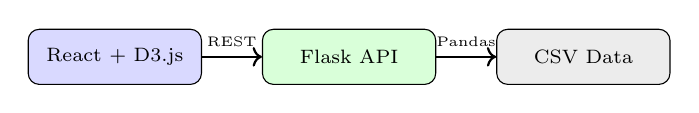
\begin{tikzpicture}[scale=0.85]
        \node[rectangle, draw, rounded corners, fill=blue!15, minimum width=2.2cm, minimum height=0.7cm, font=\scriptsize] (fe) at (-3.5,0) {React + D3.js};
        \node[rectangle, draw, rounded corners, fill=green!15, minimum width=2.2cm, minimum height=0.7cm, font=\scriptsize] (be) at (0,0) {Flask API};
        \node[rectangle, draw, rounded corners, fill=gray!15, minimum width=2.2cm, minimum height=0.7cm, font=\scriptsize] (data) at (3.5,0) {CSV Data};
        
        \draw[->, thick] (fe) -- node[above, font=\tiny] {REST} (be);
        \draw[->, thick] (be) -- node[above, font=\tiny] {Pandas} (data);
    \end{tikzpicture}
\end{frame}

\begin{frame}{Key Design Decisions}
    \begin{columns}
        \begin{column}{0.48\textwidth}
            \textbf{Visualization Choices}
            \begin{itemize}
                \item \textbf{Tabbed interface}\\
                    Separate concerns per question
                \item \textbf{Global time slider}\\
                    Consistent temporal context
                \item \textbf{Linked views}\\
                    Brushing propagates across charts
                \item \textbf{Color consistency}\\
                    Same cluster colors everywhere
                \item \textbf{Color consistency}\\
                    TODO: Add more points here
            \end{itemize}
        \end{column}
        \begin{column}{0.48\textwidth}
            \textbf{Data Processing}
            \begin{itemize}
                \item \textbf{Monthly aggregation}\\
                    Reduce 120M rows to manageable size
                \item \textbf{Caching}\\
                    Pickle cache for expensive computations
                \item TODO: Add more points here
            \end{itemize}
        \end{column}
    \end{columns}
\end{frame}

\begin{frame}{Interactive Features}
    \centering
    
    % TODO: Replace with actual screenshot showing interactivity
    \fbox{\parbox{0.8\textwidth}{\centering\vspace{2cm}\textbf{[SCREENSHOT: Interactive Features Demo]}\\\small Show hover tooltips, time slider, household filter chips\vspace{2cm}}}
    
    \vspace{10pt}
    \begin{columns}
        \begin{column}{0.3\textwidth}
            \centering
            \faMousePointer\\
            \small Hover tooltips
        \end{column}
        \begin{column}{0.3\textwidth}
            \centering
            \faSlidersH\\
            \small Time slider
        \end{column}
        \begin{column}{0.3\textwidth}
            \centering
            \faFilter\\
            \small Smart filters
        \end{column}
    \end{columns}
\end{frame}

% ==============================================================================
\section{Team Organization}
% ==============================================================================

\begin{frame}{Work Organization}
    \begin{columns}
        \begin{column}{0.55\textwidth}
            \textbf{Division of Work}
            \begin{itemize}
                \item One question per team member
                \item Shared infrastructure setup
                \item Code reviews via Git
            \end{itemize}
            
            \vspace{10pt}
            \begin{tabular}{ll}
                \textbf{Thomas} & Q1: Business Prosperity \\
                \textbf{Michal} & Q3: Employer Health \\
                \textbf{Jan} & Q2: Resident Financial Health \\
            \end{tabular}
        \end{column}
        \begin{column}{0.42\textwidth}
            \textbf{Shared Components}
            \begin{itemize}
                \item Docker infrastructure
                \item API structure
                \item Test framework
            \end{itemize}
            
            \vspace{8pt}
            \textbf{Communication}
            \begin{itemize}
                \item Regular syncs and feedback
                \item Clear API contracts
            \end{itemize}
        \end{column}
    \end{columns}
\end{frame}

\begin{frame}{Development Workflow}
    \centering
    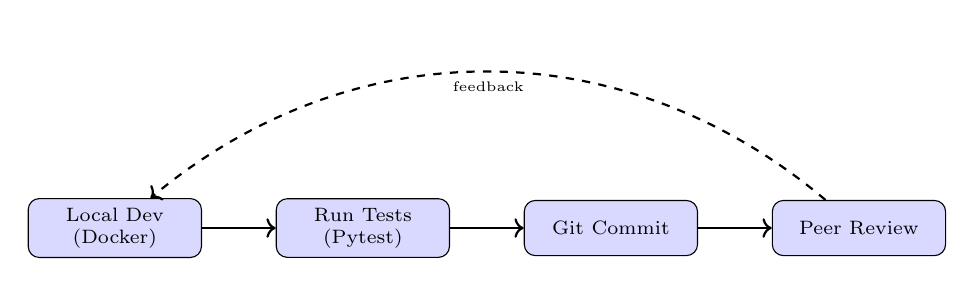
\begin{tikzpicture}[
        scale=0.9,
        box/.style={rectangle, draw, rounded corners, fill=blue!15, minimum width=2.2cm, minimum height=0.7cm, font=\scriptsize, align=center},
        arrow/.style={->, thick}
    ]
        \node[box] (dev) at (0,0) {Local Dev\\(Docker)};
        \node[box] (test) at (3.5,0) {Run Tests\\(Pytest)};
        \node[box] (commit) at (7,0) {Git Commit};
        \node[box] (review) at (10.5,0) {Peer Review};
        
        \draw[arrow] (dev) -- (test);
        \draw[arrow] (test) -- (commit);
        \draw[arrow] (commit) -- (review);
        \draw[arrow, dashed] (review) to[bend right=40] node[below, font=\tiny] {feedback} (dev);
    \end{tikzpicture}
    
    \vspace{15pt}
    \textbf{Testing Strategy}
    \begin{itemize}
        \item Backend: Pytest for each router (business, resident, employer)
        \item Docker Compose test configuration
        \item Tests run before each commit
    \end{itemize}
\end{frame}

% ==============================================================================
\section{Lessons Learned}
% ==============================================================================

\begin{frame}{Lessons Learned}
    \begin{columns}
        \begin{column}{0.48\textwidth}
            \textbf{What Worked Well}
            \begin{itemize}
                \item \textcolor{green!60!black}{\faCheck} Docker for reproducibility
                \item \textcolor{green!60!black}{\faCheck} Clear question separation
                \item \textcolor{green!60!black}{\faCheck} Caching for large datasets
                \item \textcolor{green!60!black}{\faCheck} React + D3 integration
                \item \textcolor{green!60!black}{\faCheck} Test-driven development
            \end{itemize}
        \end{column}
        \begin{column}{0.48\textwidth}
            \textbf{Challenges}
            \begin{itemize}
                \item \textcolor{red!60!black}{\faTimes} TODO
            \end{itemize}
            
            \vspace{8pt}
            \textbf{Would Do Differently}
            \begin{itemize}
                \item TODO
            \end{itemize}
        \end{column}
    \end{columns}
\end{frame}

% ==============================================================================
\section{}
% ==============================================================================

\begin{frame}{}
    \centering
    \vspace{1.5cm}
    {\Huge \textbf{Thank You!}}
    
    \vspace{1cm}
    {\large Questions?}
    
    \vspace{1cm}
    \begin{tabular}{ccc}
        Thomas Gantz & Michal Sterzel & Jan Marxen \\
        \scriptsize Q1: Business & \scriptsize Q3: Employers & \scriptsize Q2: Residents \\
    \end{tabular}
    
    \vspace{0.8cm}
    \small
    \faGithub\ \url{github.com/janmarxen/VAST-challenge}
    
    \vspace{0.5cm}
    \scriptsize
    Data Visualization -- EUMaster4HPC -- December 2025
\end{frame}

\end{document}
